\documentclass[fleqn]{jbook}
\usepackage{physpub}

\begin{document}

\begin{question}{専攻 問題4}{}
\def\Vec#1{\vec{\mathstrut #1}}
\def\Mean#1{\langle{#1}\rangle}
\def\Ca{\Atom{Ca}{20}{41}$_{21}$}
\def\Sc{\Atom{Sc}{21}{41}$_{20}$}


原子核の殻模型では、原子核の中の核子(陽子と中性子)は、他の核子からの力
の平均として、一つの引力ポテンシャルの中で独立に運動していると考える。
このポテンシャルが作るエネルギー準位に、陽子と中性子を別々に、パウリの
排他律に従ってエネルギーの低い順に詰めていくことにより、原子核が構成さ
れる。エネルギー準位間の間隔はポテンシャルの形によるが、一般に等しくは
ない。上の準位との間隔が特に大きな準位がちょうど一杯になる様な原子核は
安定であり、原子核の性質がそこで不連続に変わる。この様な原子核は閉殻を
成すという。実験によると、陽子または中性子の数が2, 8, 20, 28, 50, 82,
\ldots \ (これらの数を魔法数という)である原子核が閉殻をつくることが知ら
れている。

\begin{subquestions}
\SubQuestion
  \parbox[t]{105mm}{
  ポテンシャルによる力が中心力の場合、エネルギー準位は動径方向の波動
  関数に関する量子数$n$ と軌道角運動量$l$ (以後、角運動量は全て$\hbar$
  を単位とする)との組$(n,l)$ で指定できる。

  \begin{subsubquestions}
  \SubSubQuestion
   量子数$n$ による縮退がないとき、エネルギー準位$(n,l)$ に入り
   得る中性子の数は幾つか。中性子のスピン $s\!=\!1/2$ を考慮せよ。

  \SubSubQuestion
    中心力のポテンシャルの形を原子核の密度分布に近い形に取ると、
    低い方のエネルギー準位はおよそ、右の図の [A] のようになる
    (図では、準位が$(n,l)$ で指定してある)。このとき下から6番目まで
    の各準位にはいる中性子の個数を書け。また、閉核を成す原子核の
    中性子数は幾つになるか、小さい方から4番目まで書け。

  \end{subsubquestions}
  }\parbox[t]{55mm}{
    \vspace*{-10mm}\begin{center}
      \fbox{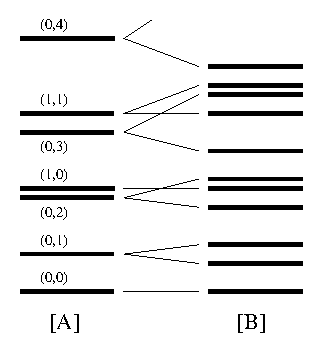
\includegraphics[clip]{1994phy4-1.eps}}
    \end{center}
  }

\SubQuestion
  中心力のポテンシャルのみでは、前問のように、28以上の魔法数を説明
  できない。そこで、前問のポテンシャルにスピン軌道相互作用の
  ポテンシャル$V_1 = -A(\Vec{l}\cdot\Vec{s})$
  を加える。ただし、$A$は正の定数とし、$\Vec{l}\ $および$\Vec{s}\ $ は
  それぞれ中性子の軌道角運動量およびスピンの演算子である。このとき、
  この中性子の全角運動量は、 $\Vec{j} = \Vec{l} + \Vec{s}\ $ と
  なり、そのエネルギー準位は、 $n,l$ と全角運動量の量子数$j$ の組
  $(n,l,j)$ で指定できる。この準位に入り得る中性子の数は、 $2j+1$
  である。

  \begin{subsubquestions}
  \SubSubQuestion
    中性子の状態 $(n,l,j)$ に関するスピン軌道相互作用の演算子 
    $(\Vec{l}\cdot\Vec{s})$ の期待値を求めよ。

  \SubSubQuestion
    スピン軌道相互作用の強さ $A$ を適当に取るとエネルギー準位は
    分離して図の [B] のようになる。下から7番目
    までの準位について低い方から順に $(n,l,j)$ を書き、それらの
    各準位に入る中性子の数を書け。
  \end{subsubquestions}

\SubQuestion
  原子核 \Ca(陽子数 $Z = 20$, 中性子数 $N = 21$) 
  と\Sc($Z = 21$, $N = 20$) の基底状態のスピン 
  (原子核全体の全角運動量) と磁気能率を、これまでの設問で考察した
  ような模型で求める。閉殻を構成している核子は、これらの量には関与
  しないとする。この問題では、磁気能率は、核磁子 $\mu_N=e\hbar/2M_p$
  を単位とする($e$ と $M_p$ は陽子の電荷と質量である)。

  \begin{subsubquestions}
  \SubSubQuestion
    原子核 \Ca と \Sc の基底状態
    のスピンを求めよ。

  \SubSubQuestion
    原子核の磁気能率の大きさ $\mu$ は、磁気能率の演算子 $\Vec{\mu}\ $
    の$z$成分の、磁気量子数 $m_j=j$ の状態での期待値と定義されている。
    状態$(n,l,j)$ の核子は、その軌道運動により $g_l\Vec{l}$ 、スピン
    により$g_s\Vec{s}\ $ の磁気能率をもつので、その磁気能率の演算子は
    これらのベクトル和%
    $\Vec{\mu}=g_l\Vec{l}+g_s\Vec{s}\ $
    となる。ただし、係数 $g_l$と$g_s$ は核子の軌道運動量とスピンの
    $g$因子と呼ばれる。演算子$\mu_z$ の状態 $(n,l,j)$ での期待値は、
    その状態での$(\Vec{\mu}\cdot\Vec{j})j_z/\Mean{\vec{j}^2}\ $ の期待値で与えられる
    ことを使って、$\Mean{\Vec{\mu}\cdot\Vec{j}}$ を $l,s,j$ と
    $g_l,g_s$ で表し、$\mu$ を求めよ。

  \SubSubQuestion
    中性子の軌道運動は中性子が電荷を持たないので磁気能率に寄与せず
    $(g_l=0)$、陽子に対しては、$g_l=1$ である。測定された中性子と
    陽子のスピンの$g$因子はそれぞれ $g_s = -3.8$、$g_s = 5.6$ である。
    原子核 \Ca と \Sc の基底状態
    の $\mu$ を計算せよ。

  \end{subsubquestions}
\end{subquestions}
\end{question}
\begin{answer}{専攻 問題4}{}
\def\Bracket#1#2#3{\langle{#1}|{#2}|{#3}\rangle}
\def\Mean#1{\langle{#1}\rangle}
\def\Vec#1{\vec{\mathstrut #1}}
\def\sqr{\,\raisebox{1ex}{\scriptsize{2}}}
\def\Ca{\Atom{Ca}{20}{41}$_{21}$}
\def\Sc{\Atom{Sc}{21}{41}$_{20}$}

\begin{subanswers}
\SubAnswer
  \begin{subsubanswers}
  \SubSubAnswer
    軌道角運動量による縮退度が$2l+1$で、それぞれに対して
    スピンによる縮退が、$2$つある。従って、$4l+2$個の中性子が入り得る。

  \SubSubAnswer
    下の準位からそれぞれ$2,6,10,2,14,6$個。閉殻をなす中性子数(魔法数)
    は、$2,8,20,40$となる。\\$(0,2)$,$(0,3)$の準位では、それぞれ
    $(1,0)$,$(1,1)$の準位と近いため閉殻を成さない。

(補足)3次元の調和振動子のエネルギー固有値は、$n'=2(n-1)+l$できま
る。$(0,2)(1,0)$の準位は$n'=0$に、$(0,3),(1,1)$の準位は$n'=1$に対
応している。この$n'$の縮退が解けて[A]のエネルギー準位が生まれたと
考えればよい。

  \end{subsubanswers}

\SubAnswer
  \begin{subsubanswers}
  \SubSubAnswer
    $\Vec{j}=\Vec{l}+\Vec{s}\ $だから、
%
    \[\Vec{j}\sqr%
        = (\Vec{l}+\Vec{s})\sqr%
        = \Vec{l}\sqr + 2\Vec{l}\cdot\Vec{s} + \Vec{s}\sqr \]
%
    従って期待値$\Mean{\Vec{l}\cdot\Vec{s}}$は、
%
    \[ \Mean{\Vec{l}\cdot\Vec{s}}%
      = \Bracket{lj}{\frac{1}{2}(\Vec{j}\sqr-\Vec{l}\sqr-\Vec{s}\sqr)}{lj}%
      = \frac{1}{2}\{j(j+1)-l(l+1)-s(s+1)\} \]
%

  \SubSubAnswer
    一次摂動の範囲でエネルギー準位は
    $-A\Mean{\Vec{l}\cdot\Vec{s}}$
    だけ変化するので、
    同じ$(n,l)$を持つ状態では、$j$ が大きい
    ($\Mean{\Vec{l}\cdot\Vec{s}}$が
    大きい)方がエネルギー準位が
    低くなる。従って、エネルギー準位とそこに入り得る中性子の数は
    低い順に以下のようになる。

    \begin{tabular}{|l|c|c|c|c|c|c|c|} \hline
      (n,l,j) & (0,0,1/2) & (0,1,3/2) & (0,1,1/2) & (0,2,5/2) & (1,0,1/2) & (0,2,3/2) & (0,3,7/2) \\ \hline
      中性子の数 & 2 & 4 & 2 & 6 & 2 & 4 & 8 \\ \hline
    \end{tabular}

    この結果、問題の図[B]から読みとれる魔法数は$2,8,20,28,...$
    となり、実験で得られている値と一致する。

  \end{subsubanswers}


\SubAnswer
  \begin{subsubanswers}
  \SubSubAnswer
    魔法数が$20$なので、どちらも、一個だけ閉殻を構成できない核子が
    余る。その核子は$(0,3,7/2)$へ入るので、スピンはどちらも$7/2$で
    ある。

  \SubSubAnswer
    まず、$\Vec{l}\cdot\Vec{j} \ $と
    $ \ \Vec{s}\cdot\Vec{j} \ $を求める。
%
    \[ \Vec{s}\sqr = (\Vec{j}-\Vec{l})\sqr%
                   = \Vec{j}\sqr-2\Vec{l}\cdot\Vec{j}+\Vec{l}\sqr \]
%
    などから、
%
    \[ \Vec{l}\cdot\Vec{j}%
       = \frac{1}{2}(\Vec{j}\sqr+\Vec{l}\sqr-\Vec{s}\sqr )%
       \hspace{10mm}%
       \Vec{s}\cdot\Vec{j}%
       =\frac{1}{2}(\Vec{j}\sqr-\Vec{l}\sqr+\Vec{s}\sqr ) \]
%
    が得られる。これを使うと、
%
    \begin{eqnarray*}
      \Vec{\mu}\cdot\Vec{j}%
        &=& g_l \Vec{l}\cdot\Vec{j} +g_s \Vec{s}\cdot\Vec{j}%
         =  g_l\frac{1}{2}(\Vec{j}\sqr+\Vec{l}\sqr-\Vec{s}\sqr )%
           +g_s\frac{1}{2}(\Vec{j}\sqr-\Vec{l}\sqr+\Vec{s}\sqr )\\
      \Mean{\Vec{\mu}\cdot\Vec{j}}%
        &=& \frac{g_l}{2}\left\{j(j+1)+l(l+1)-s(s+1)\right\}%
           +\frac{g_s}{2}\left\{j(j+1)-l(l+1)+s(s+1)\right\} \\*[2mm]
      \mu%
        &=& \Bracket{nlj(m_j=j)}{\mu_z}{nlj(m_j=j)}%
         =  \Bracket{nlj(m_j=j)}{%
              \frac{(\Vec{\mu}\cdot\Vec{j})j_z}{j(j+1)}}%
            {nlj(m_j=j)}\\
        &=& \frac{1}{j+1}\left[\frac{g_l}{2}%
            \left\{j(j+1)+l(l+1)-s(s+1)\right\}%
           +\frac{g_s}{2}%
            \left\{j(j+1)-l(l+1)+s(s+1)\right\}\right]
    \end{eqnarray*}
%

  \SubSubAnswer
    上で得た式を用いる。\Ca では、$(0,3,7/2)$
    に入る中性子が一個余っているので、
%
    \[ \mu = \frac{2}{9}\left[0+\frac{-3.8}{2}\left\{\frac{63}{4}-12+\frac{3}{4}%
             \right\}\right] = -1.9 \]
%
    となる。同様にして、\Sc では、余っているのは
    陽子なので、
%
    \[ \mu = \frac{2}{9}\left[\frac{1}{2}\left\{\frac{63}{4}+12-\frac{3}{4}%
       \right\}+\frac{5.6}{2}\left\{\frac{63}{4}-12+\frac{3}{4}
       \right\}\right] = 5.8 \]
%
    となる。

  \end{subsubanswers}
\end{subanswers}
\end{answer}

\end{document}
